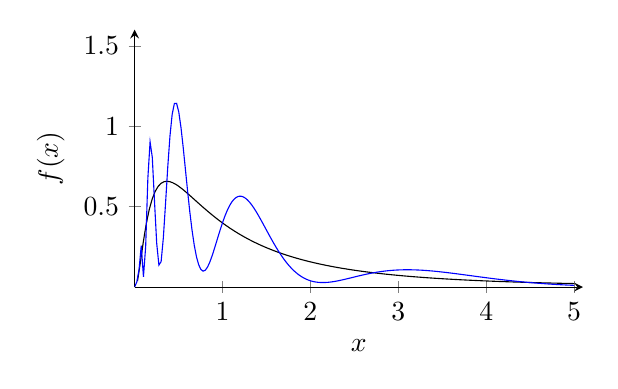
\begin{tikzpicture}
    \begin{axis}[
    axis lines=left,
    xlabel = $x$, ylabel = {$f(x)$},
    xmax = 5.1, xtick = {1, 2, 3, 4, 5},
    ymax = 1.6, ytick = {0.5, 1, 1.5},
    width=0.6\textwidth, height=0.4\textwidth]
    \addplot[domain=0:5, samples=150] {exp(-((ln(x))^2)/2)/(x*sqrt(2*pi))};
    \addplot[domain=0.001:5, samples=200, blue] {(1+0.8*sin(2*pi*(ln(\x)) r))*exp(-((ln(x))^2)/2)/(x*sqrt(2*pi))};
    \end{axis}
\end{tikzpicture}